\documentclass{article}
\usepackage[margin=0.6in]{geometry}
\usepackage{amsmath,amssymb}
\usepackage{tikz}
\usepackage{pgfplots}
\pgfplotsset{compat=1.18}
\usetikzlibrary{shapes,arrows,positioning,calc,backgrounds,fit,patterns,decorations.pathreplacing}
\usepackage{natbib}
\usepackage{graphicx}

\definecolor{cBOS}{HTML}{999999}
\definecolor{cNYC}{HTML}{0072B2}
\definecolor{cSF}{HTML}{D55E00}
\definecolor{cMUTE}{HTML}{BBBBBB}
\definecolor{cGRN}{HTML}{009E73}
\definecolor{cPNK}{HTML}{CC79A7}
\definecolor{cSKY}{HTML}{56B4E9}
\definecolor{cYEL}{HTML}{E69F00}

\pgfplotsset{
  causalre/.style={
    axis lines*=left,
    title style={font=\normalsize},
    label style={font=\small},
    tick label style={font=\scriptsize},
    legend style={font=\scriptsize, draw=none, fill=none, row sep=1pt},
    every axis plot/.append style={thick},
    axis on top,
  },
  causalre body/.style={ causalre, width=0.45\textwidth, height=6cm, },
  causalre wide/.style={ causalre, width=0.7\textwidth, height=0.6\textwidth, },
  causalre strip/.style={ causalre, width=5.0cm, height=4.5cm, title style={font=\small} },
}

\begin{document}
% v3 figures, AOAS reframe. PURE TikZ/pgfplots, matching the house `causalre`
% style (Tufte axis lines*=left, Okabe-Ito palette, manual gray CI whiskers,
% extra-tick dashed null lines, consistent marks). Coordinates emitted from
% results/ by data/scripts/make_fig_coords.py (no manual transcription).
% Figures: coverage sim, per-market forest, LEACE erasure, sensitivity (RV),
% concordance (supplement). Decomposition figure pending the pre/post-LEACE
% price re-estimate (see note at end of file).

% ======================================================================
% FIG: finite-sample coverage of the embedding-treatment DML interval
% data: results/simulation_baseline/coverage_table.csv
% ======================================================================
\begin{figure}[!htbp]
\centering
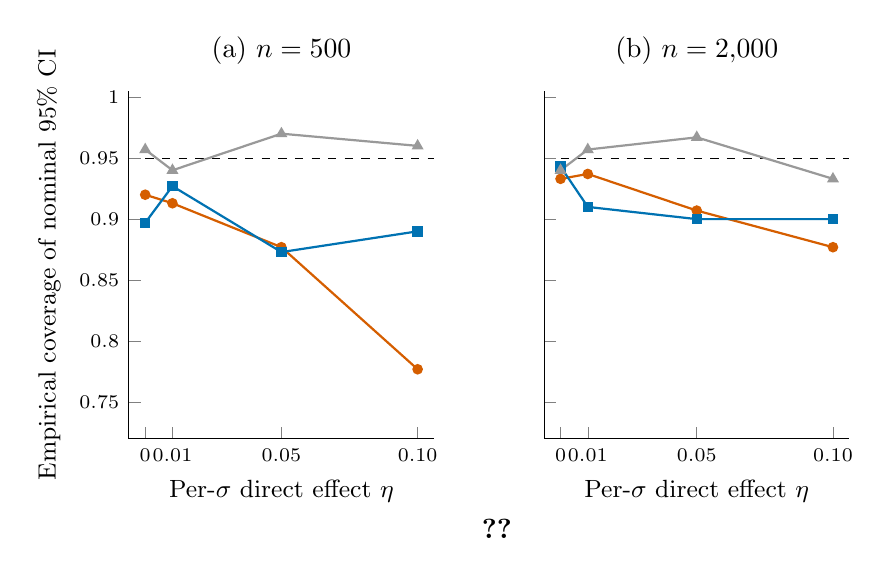
\begin{tikzpicture}
\begin{axis}[
    causalre body, name=covA,
    xlabel={Per-$\sigma$ direct effect $\eta$},
    ylabel={Empirical coverage of nominal $95\%$ CI},
    title={(a) $n = 500$},
    xmin=-0.006, xmax=0.106, ymin=0.72, ymax=1.005,
    xtick={0,0.01,0.05,0.10}, xticklabels={$0$,$0.01$,$0.05$,$0.10$},
    ytick={0.75,0.80,0.85,0.90,0.95,1.00},
    legend to name=covleg, legend columns=3,
    legend style={font=\scriptsize, draw=none, fill=none,
                  /tikz/every even column/.append style={column sep=12pt}},
    legend cell align=left,
]
\addplot[black, dashed, thin, forget plot] coordinates {(-0.006,0.95) (0.106,0.95)};
\addplot[color=cSF,  thick, mark=*,         mark size=1.5pt] coordinates {(0,0.920) (0.01,0.913) (0.05,0.877) (0.10,0.777)};
\addlegendentry{DML (in-sample PC)}
\addplot[color=cNYC, thick, mark=square*,   mark size=1.5pt] coordinates {(0,0.897) (0.01,0.927) (0.05,0.873) (0.10,0.890)};
\addlegendentry{DML (cross-fit PC)}
\addplot[color=cBOS, thick, mark=triangle*, mark size=1.7pt] coordinates {(0,0.957) (0.01,0.940) (0.05,0.970) (0.10,0.960)};
\addlegendentry{Doubly robust}
\end{axis}
\begin{axis}[
    causalre body,
    at={(covA.east)}, anchor=west, xshift=1.4cm,
    xlabel={Per-$\sigma$ direct effect $\eta$}, ylabel={},
    title={(b) $n = 2{,}000$},
    xmin=-0.006, xmax=0.106, ymin=0.72, ymax=1.005,
    xtick={0,0.01,0.05,0.10}, xticklabels={$0$,$0.01$,$0.05$,$0.10$},
    ytick={0.75,0.80,0.85,0.90,0.95,1.00}, yticklabels={,,,,,},
]
\addplot[black, dashed, thin, forget plot] coordinates {(-0.006,0.95) (0.106,0.95)};
\addplot[color=cSF,  thick, mark=*,         mark size=1.5pt, forget plot] coordinates {(0,0.933) (0.01,0.937) (0.05,0.907) (0.10,0.877)};
\addplot[color=cNYC, thick, mark=square*,   mark size=1.5pt, forget plot] coordinates {(0,0.943) (0.01,0.910) (0.05,0.900) (0.10,0.900)};
\addplot[color=cBOS, thick, mark=triangle*, mark size=1.7pt, forget plot] coordinates {(0,0.940) (0.01,0.957) (0.05,0.967) (0.10,0.933)};
\end{axis}
\node[anchor=north] at ($(covA.south east)+(0.8cm,-0.9cm)$) {\ref{covleg}};
\end{tikzpicture}
\caption{Finite-sample coverage of the nominal $95\%$ influence-function interval
for the embedding-valued treatment, across effect size $\eta$ at $n=500$ (a) and
$n=2{,}000$ (b), with $300$ Monte Carlo replications per cell. The horizontal
dashed line marks the nominal level. The in-sample principal-component DML
interval, which treats the estimated leading component as a generated regressor,
under-covers as the true effect grows, falling to $0.78$ at $n=500$, because the
orthogonal-score variance does not capture the sampling variability of the
estimated treatment direction. Forming the component out of fold (cross-fit PC)
recovers most of the lost coverage, and the doubly-robust estimator, which does
not estimate a continuous direction, is calibrated throughout but has no power
against the graded effect.}
\label{fig:sim-coverage}
\end{figure}

% ======================================================================
% FIG: per-market forest, three text channels (12 metros)
% data: shen_12city_table / baur_pooled_pca_table / counterfactual_12city_table
% rows ordered by Shen effect (idx 1 = bottom). Gray whiskers + filled dots.
% ======================================================================
\begin{figure}[!htbp]
\centering
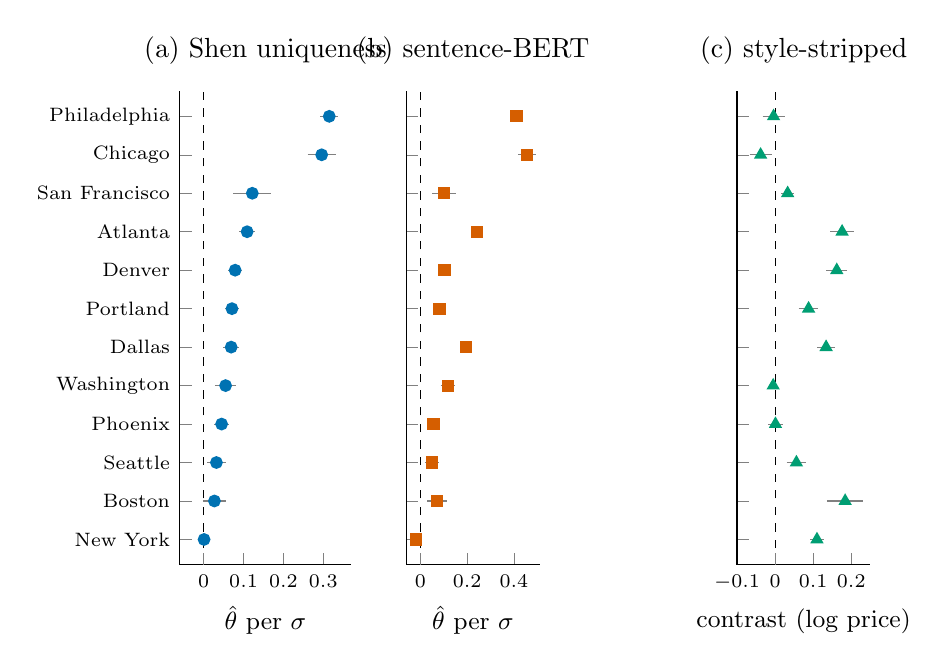
\begin{tikzpicture}
% --- panel (a) Shen uniqueness ---
\begin{axis}[
    causalre, width=0.31\textwidth, height=7.6cm, name=fsA,
    symbolic y coords={New York,Boston,Seattle,Phoenix,Washington,Dallas,Portland,Denver,Atlanta,San Francisco,Chicago,Philadelphia},
    ytick=data, y dir=normal,
    xlabel={$\hat\theta$ per $\sigma$}, xmin=-0.06, xmax=0.37,
    xtick={0,0.1,0.2,0.3}, enlarge y limits=0.06,
    title={(a) Shen uniqueness},
    extra x ticks={0}, extra x tick style={grid=major, grid style={black, dashed, thin}}, extra x tick labels={},
]
\draw[thin,gray] (axis cs:-0.011,New York)--(axis cs:0.013,New York);
\draw[thin,gray] (axis cs:-0.002,Boston)--(axis cs:0.056,Boston);
\draw[thin,gray] (axis cs:0.009,Seattle)--(axis cs:0.055,Seattle);
\draw[thin,gray] (axis cs:0.027,Phoenix)--(axis cs:0.063,Phoenix);
\draw[thin,gray] (axis cs:0.028,Washington)--(axis cs:0.082,Washington);
\draw[thin,gray] (axis cs:0.049,Dallas)--(axis cs:0.089,Dallas);
\draw[thin,gray] (axis cs:0.053,Portland)--(axis cs:0.089,Portland);
\draw[thin,gray] (axis cs:0.062,Denver)--(axis cs:0.096,Denver);
\draw[thin,gray] (axis cs:0.089,Atlanta)--(axis cs:0.129,Atlanta);
\draw[thin,gray] (axis cs:0.074,San Francisco)--(axis cs:0.170,San Francisco);
\draw[thin,gray] (axis cs:0.261,Chicago)--(axis cs:0.331,Chicago);
\draw[thin,gray] (axis cs:0.292,Philadelphia)--(axis cs:0.338,Philadelphia);
\addplot[only marks, mark=*, mark size=1.9pt, color=cNYC] coordinates {
  (0.001,New York) (0.027,Boston) (0.032,Seattle) (0.045,Phoenix) (0.055,Washington)
  (0.069,Dallas) (0.071,Portland) (0.079,Denver) (0.109,Atlanta) (0.122,San Francisco)
  (0.296,Chicago) (0.315,Philadelphia)};
\end{axis}
% --- panel (b) Baur sentence-BERT axis ---
\begin{axis}[
    causalre, width=0.27\textwidth, height=7.6cm,
    at={(fsA.east)}, anchor=west, xshift=0.7cm,
    symbolic y coords={New York,Boston,Seattle,Phoenix,Washington,Dallas,Portland,Denver,Atlanta,San Francisco,Chicago,Philadelphia},
    ytick=data, yticklabels={,,,,,,,,,,,},
    xlabel={$\hat\theta$ per $\sigma$}, xmin=-0.06, xmax=0.51,
    xtick={0,0.2,0.4}, enlarge y limits=0.06,
    title={(b) sentence-BERT},
    extra x ticks={0}, extra x tick style={grid=major, grid style={black, dashed, thin}}, extra x tick labels={},
]
\draw[thin,gray] (axis cs:-0.033,New York)--(axis cs:-0.005,New York);
\draw[thin,gray] (axis cs:0.029,Boston)--(axis cs:0.115,Boston);
\draw[thin,gray] (axis cs:0.019,Seattle)--(axis cs:0.079,Seattle);
\draw[thin,gray] (axis cs:0.030,Phoenix)--(axis cs:0.082,Phoenix);
\draw[thin,gray] (axis cs:0.087,Washington)--(axis cs:0.149,Washington);
\draw[thin,gray] (axis cs:0.175,Dallas)--(axis cs:0.215,Dallas);
\draw[thin,gray] (axis cs:0.057,Portland)--(axis cs:0.107,Portland);
\draw[thin,gray] (axis cs:0.084,Denver)--(axis cs:0.122,Denver);
\draw[thin,gray] (axis cs:0.220,Atlanta)--(axis cs:0.266,Atlanta);
\draw[thin,gray] (axis cs:0.051,San Francisco)--(axis cs:0.151,San Francisco);
\draw[thin,gray] (axis cs:0.419,Chicago)--(axis cs:0.493,Chicago);
\draw[thin,gray] (axis cs:0.390,Philadelphia)--(axis cs:0.432,Philadelphia);
\addplot[only marks, mark=square*, mark size=1.8pt, color=cSF] coordinates {
  (-0.019,New York) (0.072,Boston) (0.049,Seattle) (0.056,Phoenix) (0.118,Washington)
  (0.195,Dallas) (0.082,Portland) (0.103,Denver) (0.243,Atlanta) (0.101,San Francisco)
  (0.456,Chicago) (0.411,Philadelphia)};
\end{axis}
% --- panel (c) counterfactual style-stripped contrast ---
\begin{axis}[
    causalre, width=0.27\textwidth, height=7.6cm,
    at={(fsA.east)}, anchor=west, xshift=4.9cm,
    symbolic y coords={New York,Boston,Seattle,Phoenix,Washington,Dallas,Portland,Denver,Atlanta,San Francisco,Chicago,Philadelphia},
    ytick=data, yticklabels={,,,,,,,,,,,},
    xlabel={contrast (log price)}, xmin=-0.10, xmax=0.25,
    xtick={-0.1,0,0.1,0.2}, enlarge y limits=0.06,
    title={(c) style-stripped},
    extra x ticks={0}, extra x tick style={grid=major, grid style={black, dashed, thin}}, extra x tick labels={},
]
\draw[thin,gray] (axis cs:0.092,New York)--(axis cs:0.128,New York);
\draw[thin,gray] (axis cs:0.136,Boston)--(axis cs:0.232,Boston);
\draw[thin,gray] (axis cs:0.030,Seattle)--(axis cs:0.082,Seattle);
\draw[thin,gray] (axis cs:-0.018,Phoenix)--(axis cs:0.020,Phoenix);
\draw[thin,gray] (axis cs:-0.015,Washington)--(axis cs:0.005,Washington);
\draw[thin,gray] (axis cs:0.111,Dallas)--(axis cs:0.157,Dallas);
\draw[thin,gray] (axis cs:0.062,Portland)--(axis cs:0.114,Portland);
\draw[thin,gray] (axis cs:0.135,Denver)--(axis cs:0.189,Denver);
\draw[thin,gray] (axis cs:0.145,Atlanta)--(axis cs:0.207,Atlanta);
\draw[thin,gray] (axis cs:0.016,San Francisco)--(axis cs:0.050,San Francisco);
\draw[thin,gray] (axis cs:-0.067,Chicago)--(axis cs:-0.009,Chicago);
\draw[thin,gray] (axis cs:-0.033,Philadelphia)--(axis cs:0.025,Philadelphia);
\addplot[only marks, mark=triangle*, mark size=2.0pt, color=cGRN] coordinates {
  (0.110,New York) (0.184,Boston) (0.056,Seattle) (0.001,Phoenix) (-0.005,Washington)
  (0.134,Dallas) (0.088,Portland) (0.162,Denver) (0.176,Atlanta) (0.033,San Francisco)
  (-0.038,Chicago) (-0.004,Philadelphia)};
\end{axis}
\end{tikzpicture}
\caption{Per-market DML estimates across the twelve metropolitan areas for the
three text channels, ordered by the Shen-Ross uniqueness effect. Filled dots are
point estimates and gray whiskers are $95\%$ intervals (influence-function for
the Shen and sentence-BERT channels; coefficient-uncertainty-folded cluster
bootstrap for the counterfactual contrast). The dashed vertical line marks the
null. The sentence-BERT axis is oriented so its pooled effect is non-negative.
Numerical values appear in Tables~\ref{tab:shen-12city}, \ref{tab:baur-12city},
and \ref{tab:counterfactual-12}.}
\label{fig:forest-12}
\end{figure}

% ======================================================================
% FIG: LEACE erasure completeness (held-out ridge R^2 on lat-lon)
% data: results/leace12_igbp/leace_12city_table.csv, ordered by raw R^2
% dumbbell: gray segment raw->erased, open dot raw, filled dot erased
% ======================================================================
\begin{figure}[!htbp]
\centering
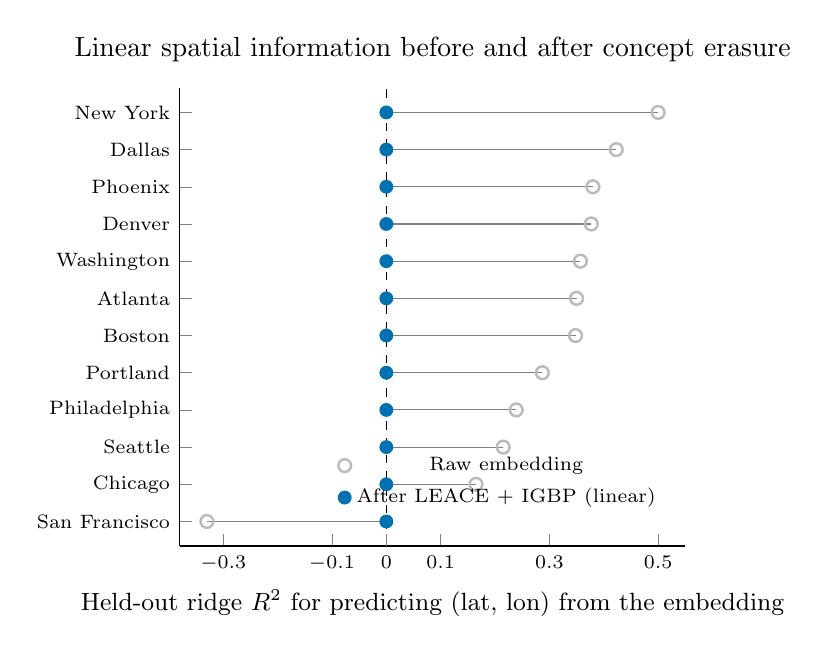
\begin{tikzpicture}
\begin{axis}[
    causalre, width=0.66\textwidth, height=7.4cm,
    symbolic y coords={San Francisco,Chicago,Seattle,Philadelphia,Portland,Boston,Atlanta,Washington,Denver,Phoenix,Dallas,New York},
    ytick=data, enlarge y limits=0.06,
    xlabel={Held-out ridge $R^2$ for predicting (lat, lon) from the embedding},
    xmin=-0.38, xmax=0.55, xtick={-0.3,-0.1,0,0.1,0.3,0.5},
    title={Linear spatial information before and after concept erasure},
    extra x ticks={0}, extra x tick style={grid=major, grid style={black, dashed, thin}}, extra x tick labels={},
    legend style={font=\scriptsize, draw=none, fill=none, at={(0.97,0.06)}, anchor=south east, row sep=1pt},
]
% raw -> erased connecting segments
\draw[thin,gray] (axis cs:-0.330,San Francisco)--(axis cs:0.000,San Francisco);
\draw[thin,gray] (axis cs:0.165,Chicago)--(axis cs:0.000,Chicago);
\draw[thin,gray] (axis cs:0.215,Seattle)--(axis cs:0.000,Seattle);
\draw[thin,gray] (axis cs:0.239,Philadelphia)--(axis cs:0.000,Philadelphia);
\draw[thin,gray] (axis cs:0.287,Portland)--(axis cs:0.000,Portland);
\draw[thin,gray] (axis cs:0.348,Boston)--(axis cs:0.000,Boston);
\draw[thin,gray] (axis cs:0.350,Atlanta)--(axis cs:0.000,Atlanta);
\draw[thin,gray] (axis cs:0.357,Washington)--(axis cs:0.000,Washington);
\draw[thin,gray] (axis cs:0.377,Denver)--(axis cs:0.000,Denver);
\draw[thin,gray] (axis cs:0.380,Phoenix)--(axis cs:0.000,Phoenix);
\draw[thin,gray] (axis cs:0.423,Dallas)--(axis cs:0.000,Dallas);
\draw[thin,gray] (axis cs:0.500,New York)--(axis cs:0.000,New York);
\addplot[only marks, mark=o, mark size=2.3pt, color=cMUTE, line width=0.9pt] coordinates {
  (-0.330,San Francisco) (0.165,Chicago) (0.215,Seattle) (0.239,Philadelphia) (0.287,Portland)
  (0.348,Boston) (0.350,Atlanta) (0.357,Washington) (0.377,Denver) (0.380,Phoenix)
  (0.423,Dallas) (0.500,New York)};
\addlegendentry{Raw embedding}
\addplot[only marks, mark=*, mark size=2.1pt, color=cNYC] coordinates {
  (0.000,San Francisco) (0.000,Chicago) (0.000,Seattle) (0.000,Philadelphia) (0.000,Portland)
  (0.000,Boston) (0.000,Atlanta) (0.000,Washington) (0.000,Denver) (0.000,Phoenix)
  (0.000,Dallas) (0.000,New York)};
\addlegendentry{After LEACE $+$ IGBP (linear)}
\end{axis}
\end{tikzpicture}
\caption{Held-out ridge $R^2$ for recovering the continuous latitude-longitude
coordinate from the sentence-BERT embedding, before (open) and after (filled)
the composed linear concept erasure, in each of the twelve markets ordered by raw
$R^2$. The raw embedding carries substantial linear spatial signal, recovering
the coordinate at $R^2$ up to $0.50$ in New York; the negative San Francisco
value reflects out-of-sample probe performance below the coordinate-mean
baseline rather than absent signal. Linear erasure drives the recoverable signal
to within Monte Carlo noise of zero in every market, the exact-guardedness
property of LEACE. Residual \emph{nonlinear} leakage, which a linear probe cannot
see, is quantified separately in Section~\ref{sec:leace-12}.}
\label{fig:erasure-12}
\end{figure}

% ======================================================================
% FIG: GRL adversarial erasure foil -- a fresh probe recovers location
% from the adversarially-deconfounded encoder but not from the LEACE projection
% data: results/adversarial_12city/adversarial_12city_summary.csv (geo_probe_r2)
% vs the LEACE linear-erased coordinate R2 (~0, fig:erasure-12)
% ======================================================================
\begin{figure}[!htbp]
\centering
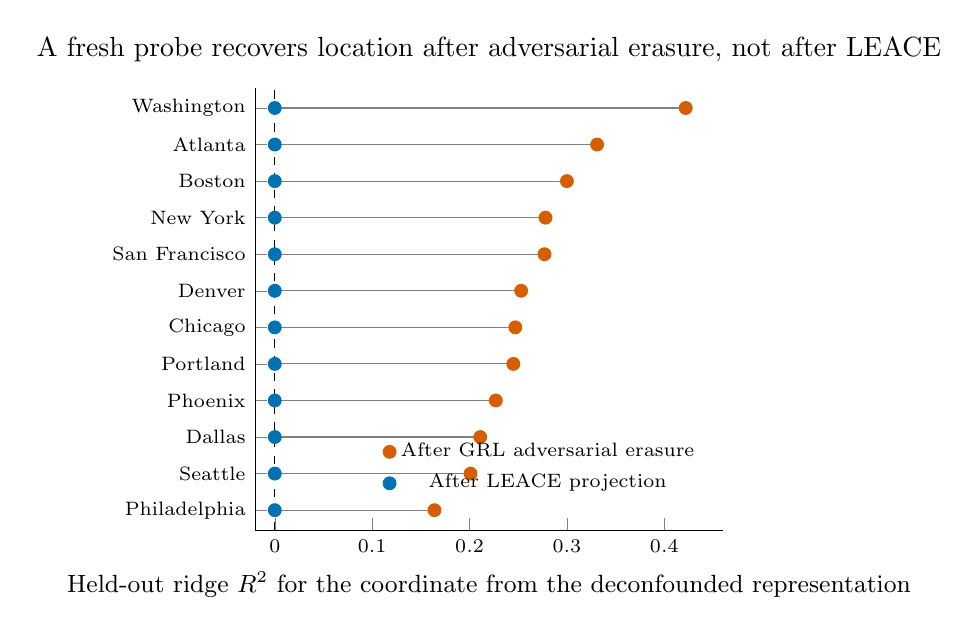
\begin{tikzpicture}
\begin{axis}[
    causalre, width=0.62\textwidth, height=7.2cm,
    symbolic y coords={Philadelphia,Seattle,Dallas,Phoenix,Portland,Chicago,
                       Denver,San Francisco,New York,Boston,Atlanta,Washington},
    ytick=data, enlarge y limits=0.05,
    xlabel={Held-out ridge $R^2$ for the coordinate from the deconfounded representation},
    xmin=-0.02, xmax=0.46, xtick={0,0.1,0.2,0.3,0.4},
    xticklabel={\pgfmathprintnumber[fixed,precision=1]{\tick}},
    title={A fresh probe recovers location after adversarial erasure, not after LEACE},
    extra x ticks={0}, extra x tick style={grid=major, grid style={black, dashed, thin}}, extra x tick labels={},
    legend style={font=\scriptsize, draw=none, fill=none, at={(0.97,0.06)}, anchor=south east, row sep=1pt},
]
\draw[thin,gray] (axis cs:0.164,Philadelphia)--(axis cs:0.000,Philadelphia);
\draw[thin,gray] (axis cs:0.201,Seattle)--(axis cs:0.000,Seattle);
\draw[thin,gray] (axis cs:0.211,Dallas)--(axis cs:0.000,Dallas);
\draw[thin,gray] (axis cs:0.227,Phoenix)--(axis cs:0.000,Phoenix);
\draw[thin,gray] (axis cs:0.245,Portland)--(axis cs:0.000,Portland);
\draw[thin,gray] (axis cs:0.247,Chicago)--(axis cs:0.000,Chicago);
\draw[thin,gray] (axis cs:0.253,Denver)--(axis cs:0.000,Denver);
\draw[thin,gray] (axis cs:0.277,San Francisco)--(axis cs:0.000,San Francisco);
\draw[thin,gray] (axis cs:0.278,New York)--(axis cs:0.000,New York);
\draw[thin,gray] (axis cs:0.300,Boston)--(axis cs:0.000,Boston);
\draw[thin,gray] (axis cs:0.331,Atlanta)--(axis cs:0.000,Atlanta);
\draw[thin,gray] (axis cs:0.422,Washington)--(axis cs:0.000,Washington);
\addplot[only marks, mark=*, mark size=2.1pt, color=cSF] coordinates {
  (0.164,Philadelphia) (0.201,Seattle) (0.211,Dallas) (0.227,Phoenix) (0.245,Portland)
  (0.247,Chicago) (0.253,Denver) (0.277,San Francisco) (0.278,New York) (0.300,Boston)
  (0.331,Atlanta) (0.422,Washington)};
\addlegendentry{After GRL adversarial erasure}
\addplot[only marks, mark=*, mark size=2.1pt, color=cNYC] coordinates {
  (0.000,Philadelphia) (0.000,Seattle) (0.000,Dallas) (0.000,Phoenix) (0.000,Portland)
  (0.000,Chicago) (0.000,Denver) (0.000,San Francisco) (0.000,New York) (0.000,Boston)
  (0.000,Atlanta) (0.000,Washington)};
\addlegendentry{After LEACE projection}
\end{axis}
\end{tikzpicture}
\caption{The frozen-probe diagnostic applied to two erasure methods, in each of the
twelve markets. A ridge probe of the latitude-longitude coordinate is trained from
scratch on the deconfounded representation. Against the gradient-reversal
adversarial encoder, whose own multi-head discriminator has been driven to chance
on location (out-of-sample coordinate $R^2 \le 0.07$ across the panel), the fresh
probe still recovers the coordinate at $R^2$ between $0.16$ and $0.42$; against the
LEACE projection the same probe sits at the chance baseline, the exact-guardedness
property of closed-form erasure. The adversarial training did not remove location,
it taught its discriminator not to look, which is the saddle of
Proposition~\ref{prop:frozen_probe}(c) realized across every market.}
\label{fig:grl-foil}
\end{figure}

% ======================================================================
% FIG: per-market robustness value (sensitivity to unmeasured confounding)
% data: results/replications/confounder_sensitivity_12.csv (rv, block=none)
% ======================================================================
\begin{figure}[!htbp]
\centering
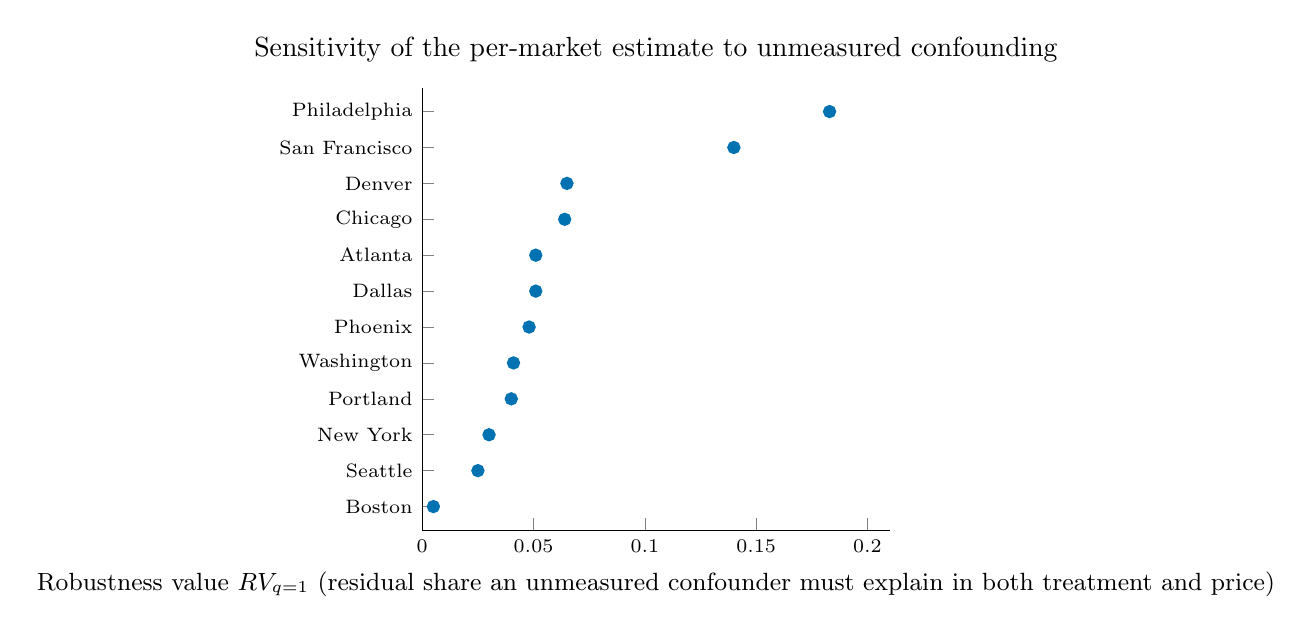
\begin{tikzpicture}
\begin{axis}[
    causalre, width=0.62\textwidth, height=7.2cm,
    symbolic y coords={Boston,Seattle,New York,Portland,Washington,Phoenix,Dallas,Atlanta,Chicago,Denver,San Francisco,Philadelphia},
    ytick=data, enlarge y limits=0.06,
    xlabel={Robustness value $RV_{q=1}$ (residual share an unmeasured confounder must explain in both treatment and price)},
    xmin=0, xmax=0.21, xtick={0,0.05,0.10,0.15,0.20},
    xticklabel={\pgfmathprintnumber[fixed,precision=2]{\tick}},
    title={Sensitivity of the per-market estimate to unmeasured confounding},
]
\addplot[only marks, mark=*, mark size=2.0pt, color=cNYC] coordinates {
  (0.005,Boston) (0.025,Seattle) (0.030,New York) (0.040,Portland) (0.041,Washington)
  (0.048,Phoenix) (0.051,Dallas) (0.051,Atlanta) (0.064,Chicago) (0.065,Denver)
  (0.140,San Francisco) (0.183,Philadelphia)};
\end{axis}
\end{tikzpicture}
\caption{Robustness value for each market's sentence-BERT effect, the share of
residual variance an unmeasured confounder would need to explain in both the
treatment and log price to drive the estimate to zero, following
\citet{cinelli2020making}. Larger values are more robust. The estimate is most
robust in Philadelphia ($0.18$) and San Francisco ($0.14$) and most fragile in
the markets whose point estimates are already near zero. The modest robustness
values in several markets are the reason we read the per-market estimates as
associational and sensitivity-bounded rather than cleanly causal.}
\label{fig:sensitivity-rv}
\end{figure}

% ======================================================================
% SUPPLEMENT FIG: cross-method concordance scatter (Shen vs Baur), r = 0.94
% data: results/replications/cross_method_concordance.csv
% ======================================================================
\begin{figure}[!htbp]
\centering
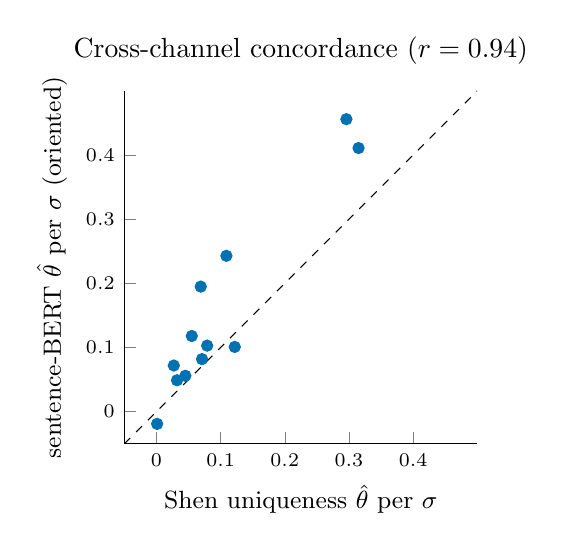
\begin{tikzpicture}
\begin{axis}[
    causalre, width=0.5\textwidth, height=0.5\textwidth,
    axis equal image,
    xlabel={Shen uniqueness $\hat\theta$ per $\sigma$},
    ylabel={sentence-BERT $\hat\theta$ per $\sigma$ (oriented)},
    xmin=-0.05, xmax=0.50, ymin=-0.05, ymax=0.50,
    xtick={0,0.1,0.2,0.3,0.4}, ytick={0,0.1,0.2,0.3,0.4},
    title={Cross-channel concordance ($r = 0.94$)},
]
\addplot[black, dashed, thin, forget plot] coordinates {(-0.05,-0.05) (0.50,0.50)};
\addplot[only marks, mark=*, mark size=1.8pt, color=cNYC] coordinates {
  (0.027,0.072) (0.001,-0.019) (0.122,0.101) (0.055,0.118) (0.315,0.411) (0.296,0.456)
  (0.032,0.049) (0.079,0.103) (0.109,0.243) (0.071,0.082) (0.045,0.056) (0.069,0.195)};
\end{axis}
\end{tikzpicture}
\caption{Per-market estimates of the two embedding channels against each other,
with the $45^\circ$ identity line. The two channels co-move almost perfectly
across markets (Pearson $r = 0.94$), so they recover one underlying signal under
two encodings rather than two independent measurements; the systematic departure
from the identity line reflects that the sentence-BERT axis is roughly twice the
Shen channel in magnitude, not a difference in which markets carry the signal.}
\label{fig:concordance}
\end{figure}

% ======================================================================
% FIG (headline): is the text-price effect spatially confounded?
% Gelbach fixed-treatment toggle: hold PC1 fixed, add a location basis to the
% confounders. (a) effect without vs with spatial adjustment (dumbbell); they
% barely move -> small confounded share. (b) PC1 geography R^2 -> the text IS
% geographic, so panel (a)'s robustness is non-vacuous.
% data: results/replications/leace_price_decomposition.csv
% ======================================================================
\begin{figure}[!htbp]
\centering
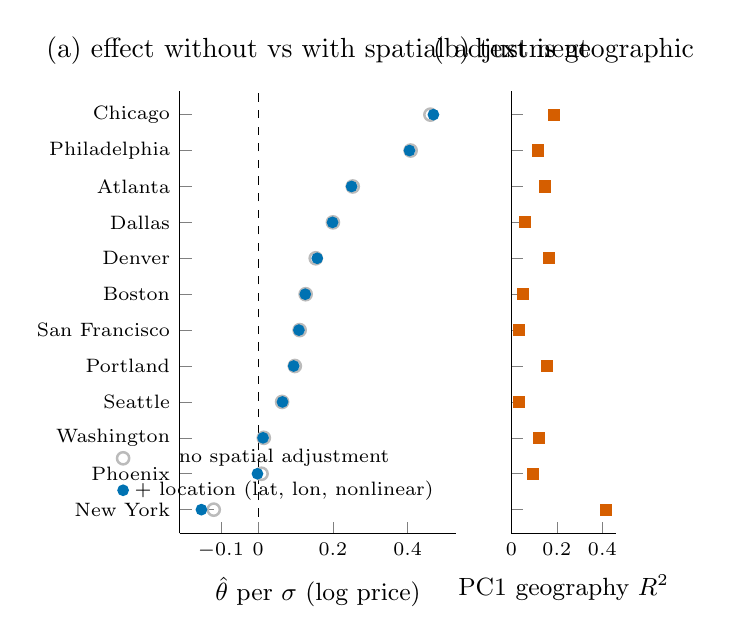
\begin{tikzpicture}
\begin{axis}[
    causalre, width=0.42\textwidth, height=7.2cm, name=dcA,
    symbolic y coords={New York,Phoenix,Washington,Seattle,Portland,San Francisco,Boston,Denver,Dallas,Atlanta,Philadelphia,Chicago},
    ytick=data, enlarge y limits=0.06,
    xlabel={$\hat\theta$ per $\sigma$ (log price)}, xmin=-0.21, xmax=0.53,
    xtick={-0.1,0,0.2,0.4},
    title={(a) effect without vs with spatial adjustment},
    extra x ticks={0}, extra x tick style={grid=major, grid style={black, dashed, thin}}, extra x tick labels={},
    legend style={font=\scriptsize, draw=none, fill=none, at={(0.97,0.05)}, anchor=south east, row sep=1pt},
]
\draw[thin,gray] (axis cs:-0.119,New York)--(axis cs:-0.152,New York);
\draw[thin,gray] (axis cs:0.009,Phoenix)--(axis cs:-0.002,Phoenix);
\draw[thin,gray] (axis cs:0.015,Washington)--(axis cs:0.013,Washington);
\draw[thin,gray] (axis cs:0.064,Seattle)--(axis cs:0.065,Seattle);
\draw[thin,gray] (axis cs:0.098,Portland)--(axis cs:0.095,Portland);
\draw[thin,gray] (axis cs:0.111,San Francisco)--(axis cs:0.109,San Francisco);
\draw[thin,gray] (axis cs:0.127,Boston)--(axis cs:0.126,Boston);
\draw[thin,gray] (axis cs:0.154,Denver)--(axis cs:0.158,Denver);
\draw[thin,gray] (axis cs:0.200,Dallas)--(axis cs:0.199,Dallas);
\draw[thin,gray] (axis cs:0.253,Atlanta)--(axis cs:0.250,Atlanta);
\draw[thin,gray] (axis cs:0.408,Philadelphia)--(axis cs:0.405,Philadelphia);
\draw[thin,gray] (axis cs:0.461,Chicago)--(axis cs:0.469,Chicago);
\addplot[only marks, mark=o, mark size=2.2pt, color=cMUTE, line width=0.9pt] coordinates {
  (-0.119,New York) (0.009,Phoenix) (0.015,Washington) (0.064,Seattle) (0.098,Portland)
  (0.111,San Francisco) (0.127,Boston) (0.154,Denver) (0.200,Dallas) (0.253,Atlanta)
  (0.408,Philadelphia) (0.461,Chicago)};
\addlegendentry{no spatial adjustment}
\addplot[only marks, mark=*, mark size=1.7pt, color=cNYC] coordinates {
  (-0.152,New York) (-0.002,Phoenix) (0.013,Washington) (0.065,Seattle) (0.095,Portland)
  (0.109,San Francisco) (0.126,Boston) (0.158,Denver) (0.199,Dallas) (0.250,Atlanta)
  (0.405,Philadelphia) (0.469,Chicago)};
\addlegendentry{$+$ location (lat, lon, nonlinear)}
\end{axis}
\begin{axis}[
    causalre, width=0.24\textwidth, height=7.2cm,
    at={(dcA.east)}, anchor=west, xshift=0.7cm,
    symbolic y coords={New York,Phoenix,Washington,Seattle,Portland,San Francisco,Boston,Denver,Dallas,Atlanta,Philadelphia,Chicago},
    ytick=data, yticklabels={,,,,,,,,,,,},
    xlabel={PC1 geography $R^2$}, xmin=0, xmax=0.46, xtick={0,0.2,0.4},
    enlarge y limits=0.06,
    title={(b) text is geographic},
]
\addplot[only marks, mark=square*, mark size=1.8pt, color=cSF] coordinates {
  (0.417,New York) (0.097,Phoenix) (0.121,Washington) (0.034,Seattle) (0.158,Portland)
  (0.035,San Francisco) (0.053,Boston) (0.165,Denver) (0.059,Dallas) (0.148,Atlanta)
  (0.116,Philadelphia) (0.187,Chicago)};
\end{axis}
\end{tikzpicture}
\caption{Is the per-market text-price effect spatially confounded? Holding the
leading text principal component fixed as the treatment, panel (a) plots its DML
effect on log price controlling for the structured confounders without (open) and
with (filled) a location adjustment that adds latitude, longitude, and their
quadratic and interaction terms to the confounder set. The two estimates nearly
coincide in eleven of twelve markets, with a confounded share below five percent
of the effect; New York is the exception, where the location adjustment moves the
estimate by about a quarter of its magnitude without changing its sign. Panel (b)
reports the share of the treatment's own variance that the location basis
explains, which reaches $0.42$ in New York and exceeds $0.10$ in six markets, so
the robustness in panel (a) is not an artifact of a treatment that carries no
geography: the text direction does encode location, yet that location component
does not drive its price effect.}
\label{fig:decomposition}
\end{figure}

\end{document}
